% Appendix Template

\chapter{Results of experiment 1.1} % Main appendix title

\label{Appendix1-1} % Change X to a consecutive letter; for referencing this appendix elsewhere, use \ref{AppendixX}

\begin{figure}[th]
\centering
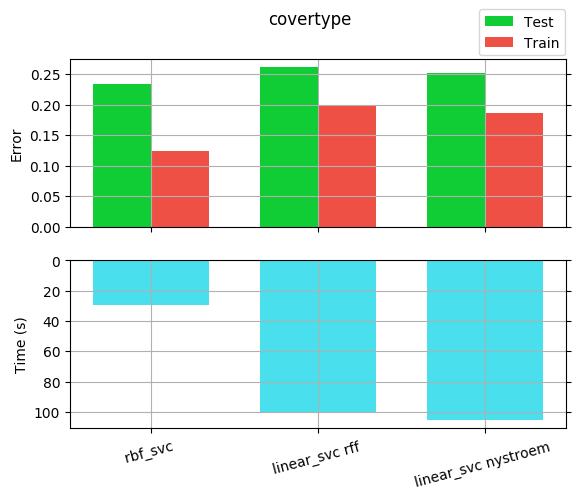
\includegraphics[scale=\imgscale]{Figures/1_1/covertype}
\decoRule
\caption[1.1 covertype]{RBF-SVM and Linear-SVM with RFF and \Nys}
\label{fig:1_1_covertype}
\end{figure}

\begin{figure}[th]
\centering
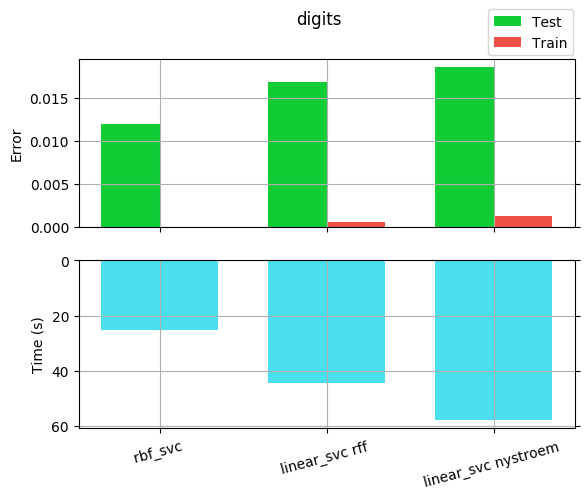
\includegraphics[scale=\imgscale]{Figures/1_1/digits}
\decoRule
\caption[1.1 digits]{RBF-SVM and Linear-SVM with RFF and \Nys}
\label{fig:1_1_digits}
\end{figure}

\begin{figure}[th]
\centering
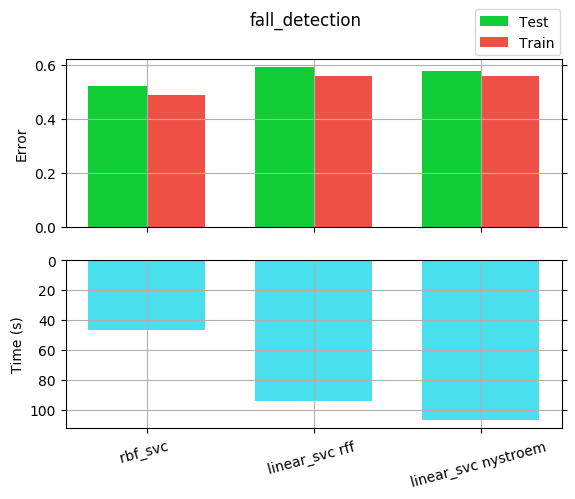
\includegraphics[scale=\imgscale]{Figures/1_1/fall_detection}
\decoRule
\caption[1.1 fall\tu detection]{RBF-SVM and Linear-SVM with RFF and \Nys}
\label{fig:1_1_fall_detection}
\end{figure}

\begin{figure}[th]
\centering
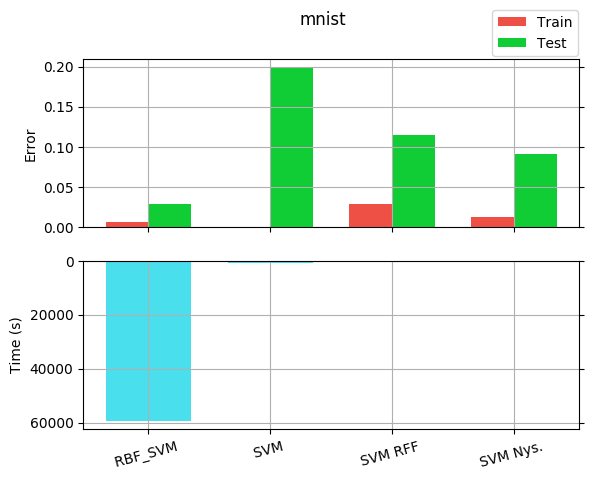
\includegraphics[scale=\imgscale]{Figures/1_1/mnist}
\decoRule
\caption[1.1 mnist]{RBF-SVM and Linear-SVM with RFF and \Nys}
\label{fig:1_1_mnist}
\end{figure}

\begin{figure}[th]
\centering
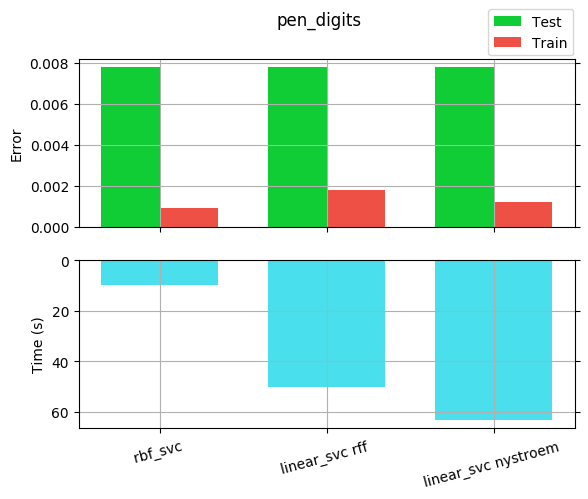
\includegraphics[scale=\imgscale]{Figures/1_1/pen_digits}
\decoRule
\caption[1.1 pen\tu digits]{RBF-SVM and Linear-SVM with RFF and \Nys}
\label{fig:1_1_pen_digits}
\end{figure}

\begin{figure}[th]
\centering
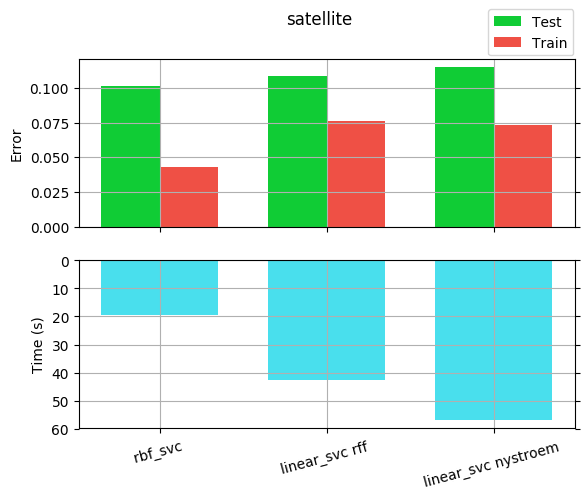
\includegraphics[scale=\imgscale]{Figures/1_1/satellite}
\decoRule
\caption[1.1 satellite]{RBF-SVM and Linear-SVM with RFF and \Nys}
\label{fig:1_1_satellite}
\end{figure}

\begin{figure}[th]
\centering
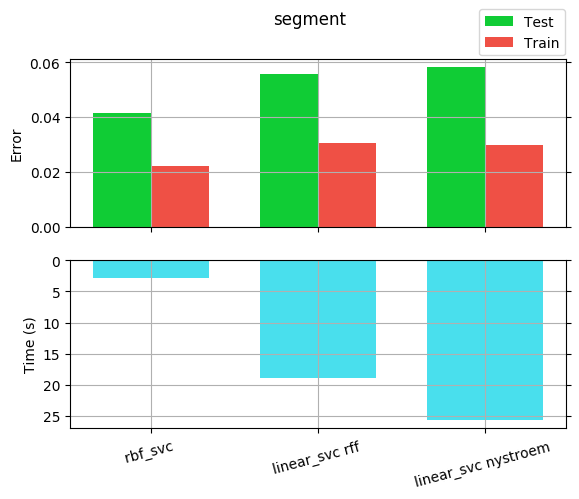
\includegraphics[scale=\imgscale]{Figures/1_1/segment}
\decoRule
\caption[1.1 segment]{RBF-SVM and Linear-SVM with RFF and \Nys}
\label{fig:1_1_segment}
\end{figure}

\begin{figure}[th]
\centering
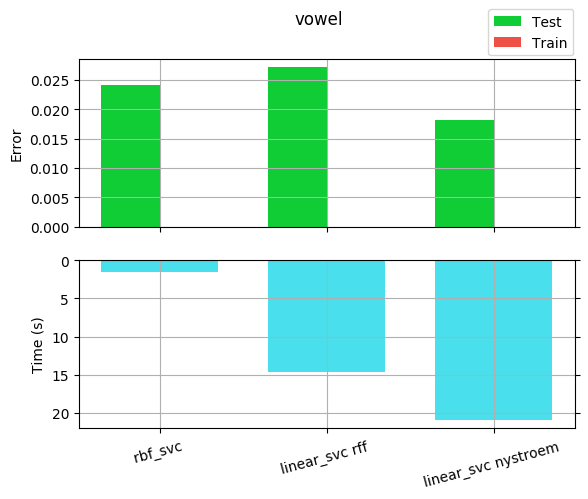
\includegraphics[scale=\imgscale]{Figures/1_1/vowel}
\decoRule
\caption[1.1 vowel]{RBF-SVM and Linear-SVM with RFF and \Nys}
\label{fig:vowel}
\end{figure}
